% If problems with the headers:
% get headings in appendix etc. right with
% \markboth{\spacedlowsmallcaps{Appendix}}{\spacedlowsmallcaps{Appendix}}
%==============================================================================
\chapter{Techniques validation}\label{cha:chapterA}
%==============================================================================

%
%
%
\section{GPE-based GSA technique validation using analytic solutions for Sobol' indices of test functions}\label{chA:GPE-based_GSA_technique_validation_using_analytic_solutions_for_Sobol'_indices_of_test_functions}
We validated the GPE-based GSA technique by emulating test functions whose Sobol' sensitivity indices can be calculated analytically. After training, the emulators were used to estimate the Sobol' indices and the estimates were compared with the corresponding known theoretical values.

%
%
%
\subsection{Ishigami function}
The Ishigami function is a function of...
%
\begin{align}\label{eq:ishigamifun}
	& Y = \sin{X_1} + a\,\sin^2{X_2} + b\,X_3^4\sin{X_1}\,,\quad\text{with} \\
	& X_i\,\,\sim\,\,\mathcal{U}([-\pi,\,\pi])\quad \text{for}\quad i=1,2,3\quad \text{and}\quad a,b>0
\end{align}

\vspace{0.2cm}\noindent
The model total variance is given in terms of $a$ and $b$ model parameters as:
%
\begin{equation}\label{eq:ifun_total_var}
	V = \frac{1}{2} + a^2\,\frac{1}{8} + b\,\frac{\pi^4}{5} + b^2\,\frac{\pi^8}{18}
\end{equation}

\vspace{0.2cm}\noindent
Sobol' sensitivity indices can be then calculated by dividing the partial variances (which are also given in terms of $a$ and $b$ parameters) by the total variance of equation~\eqref{eq:ifun_total_var}:
%
\begin{align}
	& S_{1} = \frac{V_{1}}{V},\quad V_{1} = \frac{1}{2} + b\,\frac{\pi^4}{5} + b^2\,\frac{\pi^8}{50} \\
	& S_{2} = \frac{V_{2}}{V},\quad V_{2} = a^2\,\frac{1}{8} \\
	& S_{3} = \frac{V_{3}}{V},\quad V_{3} = 0
\end{align}

\begin{align}
	& S_{T1} = \frac{V_{T1}}{V},\quad V_{T1} = \frac{1}{2}\left(1+b\,\frac{\pi^4}{5}\right)^2 + b^2\,\frac{8\pi^8}{255} \\
	& S_{T2} = \frac{V_{T2}}{V},\quad V_{T2} = V_2 \\
	& S_{T3} = \frac{V_{T3}}{V},\quad V_{T3} = b^2\,\frac{8\pi^8}{255}
\end{align}

%
%
%
\subsection{G*-function}
The G*-function is an extension of the Sobol' G-function proposed for...
%
\begin{align}\label{eq:sobolgfun}
	& Y = \prod_{i=1}^{k}g_i(X_i),\quad\text{with} \\
	& g_i(X_i)=\frac{(1+\alpha_i)\vert 2(X_i+\delta_i-I[X_i+\delta_i])-1\vert^{\alpha_i}+a_i}{1+a_i}\quad\text{and} \\
	& X_i\,\,\sim\,\,\mathcal{U}([0,\,1]),\,\,\alpha_i > 0,\,\,\delta_i\in [0,\,1],\,\,a_i>0\quad\text{for}\,\,i=1,\dots,k
\end{align}

\vspace{0.2cm}\noindent
where $I[X_i+\delta_i]$ indicates the integer part of $X_i+\delta_i$. A low $a_i$ coefficient means important $X_i$ factor, while a high $a_i$ coefficients means negligible $X_i$ effect. If more than one $a_i$ coefficient is low, higher order interaction effects will be present as well. $\delta_i$ is a shift parameter, while $\alpha_i$ is a curvature parameter.

\vspace{0.2cm}
The partial variances of the first order are given in terms of the curvature parameters $\alpha_i$s and of the $a_i$s coefficients, while the partial total variances can be calculated as a function of the first-order ones:
%
\begin{align}
	& V_i = \frac{\alpha_i^2}{(1+2\alpha_i)(1 + a_i)^2}\,,\quad\text{for}\quad i=1,\dots,k \label{eq:gfun_partial_var_first}\\
	& V_{Ti} = V_i \prod_{j=1,\,j\neq i}^{k}(1 + V_j)\,,\quad\text{for}\quad i=1,\dots,k \label{eq:gfun_partial_var_total}
\end{align}

\vspace{0.2cm}\noindent
Sobol' sensitivity indices can be then calculated by dividing the partial variances of equations~\eqref{eq:gfun_partial_var_first}--\eqref{eq:gfun_partial_var_total} by the total variance, which is again given as a function of the first-order partial variances as:
%
\begin{align}
	& S_i = \frac{V_i}{V} \quad\text{and}\quad S_{Ti} = \frac{V_{Ti}}{V} \quad\text{for}\quad i=1,\dots,k,\,\quad\text{with} \\
	& V = -1 + \prod_{i=1}^{k}(1 + V_i) 
\end{align}

%
%
%
\subsection{Simulator estimates}

\begin{table}[ht!]
    \myfloatalign
    \begin{tabularx}{\textwidth}{XXX}
    \toprule
    \tableheadline{Input factor} & \multicolumn{2}{c}{\spacedlowsmallcaps{Sobol' sensitivity index}} \\
    \midrule   
    & \tableheadline{$S_{i}$} & \tableheadline{$S_{Ti}$} \\
    \cmidrule{2-3}
    $X_{1}$ & $0.3139$ & $0.5576$ \\
    $X_{2}$ & $0.4424$ & $0.4424$ \\
    $X_{3}$ & $0.0000$ & $0.2437$ \\
    \bottomrule
    \end{tabularx}
    \caption{Ishigami function Sobol' first-order and total effects' theoretical values for $a=7,\,b=0.1$.}
    \label{tab:ifun_theo_vals}
\end{table}

\begin{table}[ht!]
    \myfloatalign
    \begin{tabularx}{\textwidth}{XXX}
    \toprule
    \tableheadline{Input factor} & \multicolumn{2}{c}{\spacedlowsmallcaps{Sobol' sensitivity index}} \\
    \midrule   
    & \tableheadline{$S_{i}$} & \tableheadline{$S_{Ti}$} \\
    \cmidrule{2-3}
    $X_{1}$   & $0.5607$ & $0.6705$ \\
    $X_{2}$   & $0.1402$ & $0.2063$ \\
    $X_{3}$   & $0.0623$ & $0.0958$ \\
    $X_{4}$   & $0.0350$ & $0.0547$ \\
    $X_{5}$   & $0.0224$ & $0.0353$ \\
    $X_{6}$   & $0.0156$ & $0.0246$ \\
    $X_{7}$   & $0.0114$ & $0.0181$ \\
    $X_{8}$   & $0.0088$ & $0.0139$ \\
    $X_{9}$   & $0.0069$ & $0.0110$ \\
    $X_{10}$  & $0.0056$ & $0.0089$ \\
    \bottomrule
    \end{tabularx}
    \caption{G*-function Sobol' first-order and total effects' theoretical values for $k=10$, $\alpha_i=1$, $\delta_i\,\,\sim\,\,\mathcal{U}([0,\,1])$, $a_i=i-1$, for $i=1,\dots,k$.}
    \label{tab:gfun_theo_vals}
\end{table}

\begin{table}[ht!]
    \myfloatalign
    \begin{tabularx}{0.8\textwidth}{lX}
    \toprule
    \tableheadline{Multiplicative factor} & \tableheadline{$R^2$ score} \\
    \midrule
    $10\times$   & $0.3796$ \\
    $20\times$   & $0.5187$ \\
    $30\times$   & $0.5438$ \\
    $40\times$   & $0.8563$ \\
    $50\times$   & $0.9526$ \\
    $60\times$   & $0.9770$ \\
    $70\times$   & $0.9806$ \\
    $80\times$   & $0.9862$ \\
    $90\times$   & $0.9876$ \\
    $100\times$  & $0.9941$ \\
    \bottomrule
    \end{tabularx}
    \caption{Ishigami function emulators' predictivity as described by the $R^2$ score.}
    \label{tab:ifun_scores}
\end{table}

\begin{table}[ht!]
    \myfloatalign
    \begin{tabularx}{0.8\textwidth}{lX}
    \toprule
    \tableheadline{Multiplicative factor} & \tableheadline{$R^2$ score} \\
    \midrule
    $10\times$   & $0.6470$ \\
    $20\times$   & $0.7689$ \\
    $30\times$   & $0.7534$ \\
    $40\times$   & $0.7881$ \\
    $50\times$   & $0.8332$ \\
    $60\times$   & $0.8396$ \\
    $70\times$   & $0.8427$ \\
    $80\times$   & $0.8569$ \\
    $90\times$   & $0.8805$ \\
    $100\times$  & $0.8896$ \\
    \bottomrule
    \end{tabularx}
    \caption{G*-function scores.}
    \label{tab:gfun_scores}
\end{table}




%
%
%
\subsection{Emulator estimates}


%
%
%
\section{HM validation using syntatic data}\label{chA:HM_validation_using_syntatic_data}
We validated HM technique against \textit{synthetic data}, generated using the \textit{in silico} model of SHAM rat heart contraction mechanics (Section~\ref{sec:ch4ratheartcontractionmodel}).

\vspace{0.2cm}
For this purpose, we started from the performed HM on the SHAM model (Section~\ref{sec:ch4modelfitting}, Figure~\ref{fig:shamhm}). We selected an intermediate wave, specifically wave $4$, among the total $8$ waves the full process took to complete (Figure~\ref{fig:hm1}). We then sampled $256$ points in wave $4$ that did not belong to the final wave, namely wave $8$ (Figures~\ref{fig:hm2}--\ref{fig:hm3}). We then simulated all these points and computed the LV features' mean and standard deviation values for the ones that led to a converging simulation ($48$ points). We further used these mean and standard deviation values as synthetic data to be matched. The LV features' synthetic variability is summarised in Table~\ref{tab:values2match4synt}.

\begin{table}[ht!]
    \myfloatalign
    \begin{tabularx}{\textwidth}{lXX}
    \toprule
    \tableheadline{LV feature} & \tableheadline{Units}                  & \tableheadline{Synthetic variability} \\
    \midrule
    $\textrm{EDV}^{*}$         & $\SI{}{\micro\liter}$                  & $493.10 \pm 16.85$ \\
    $\textrm{ESV}^{*}$         & $\SI{}{\micro\liter}$                  & $204.29 \pm  7.93$ \\
    $\textrm{EF}$              & $\SI{}{\percent}$                      & $ 58.54 \pm  1.74$ \\
    $\textrm{IVCT}$            & $\SI{}{\milli\second}$                 & $140.86 \pm  0.78$ \\
    $\textrm{ET}^{*}$          & $\SI{}{\milli\second}$                 & $ 56.77 \pm  1.53$ \\
    $\textrm{IVRT}^{*}$        & $\SI{}{\milli\second}$                 & $ 20.03 \pm  2.43$ \\
    $\textrm{Tdiast}$          & $\SI{}{\milli\second}$                 & $ 94.07 \pm  1.11$ \\
    $\textrm{PeakP}^{*}$       & $\SI{}{\kilo\pascal}$                  & $ 18.56 \pm  1.14$ \\
    $\textrm{Tpeak}$           & $\SI{}{\milli\second}$                 & $ 39.39 \pm  1.36$ \\ 
    $\textrm{ESP}$             & $\SI{}{\kilo\pascal}$                  & $ 8.74  \pm  0.21$ \\
    $\textrm{maxdP}^{*}$       & $\SI{}{\kilo\pascal\per\milli\second}$ & $ 1.08  \pm  0.06$ \\
    $\textrm{mindP}^{*}$       & $\SI{}{\kilo\pascal\per\milli\second}$ & $-0.54  \pm  0.06$ \\
    \bottomrule
    \end{tabularx}
    \caption{Synthetic data LV features' variability given as mean $\pm$ standard deviation values to match for HM validation. Only the LV features with an asterisk $(\,\,)^*$ were used as targets for HM.}
    \label{tab:values2match4synt}
\end{table}

\vspace{0.2cm}
We started the HM process from the same initial space-filling design (lightest blue variant coloured points in Figure~\ref{fig:shamhm}) used for the SHAM model HM, this time trying to match the synthetic data instead of the experimental data. To replicate exactly the same process, we tried to match the same $7$ features out of the total $12$ features of interest, although we had mean and standard deviation values for all the LV features. Figure~\ref{fig:syntfeatmatch} shows that all the LV features were perfectly matched at the end of the HM process (which took $9$ waves to complete), including the $5$ features we did not directly selected as targets for HM.

\begin{figure}[ht!]
    \myfloatalign
    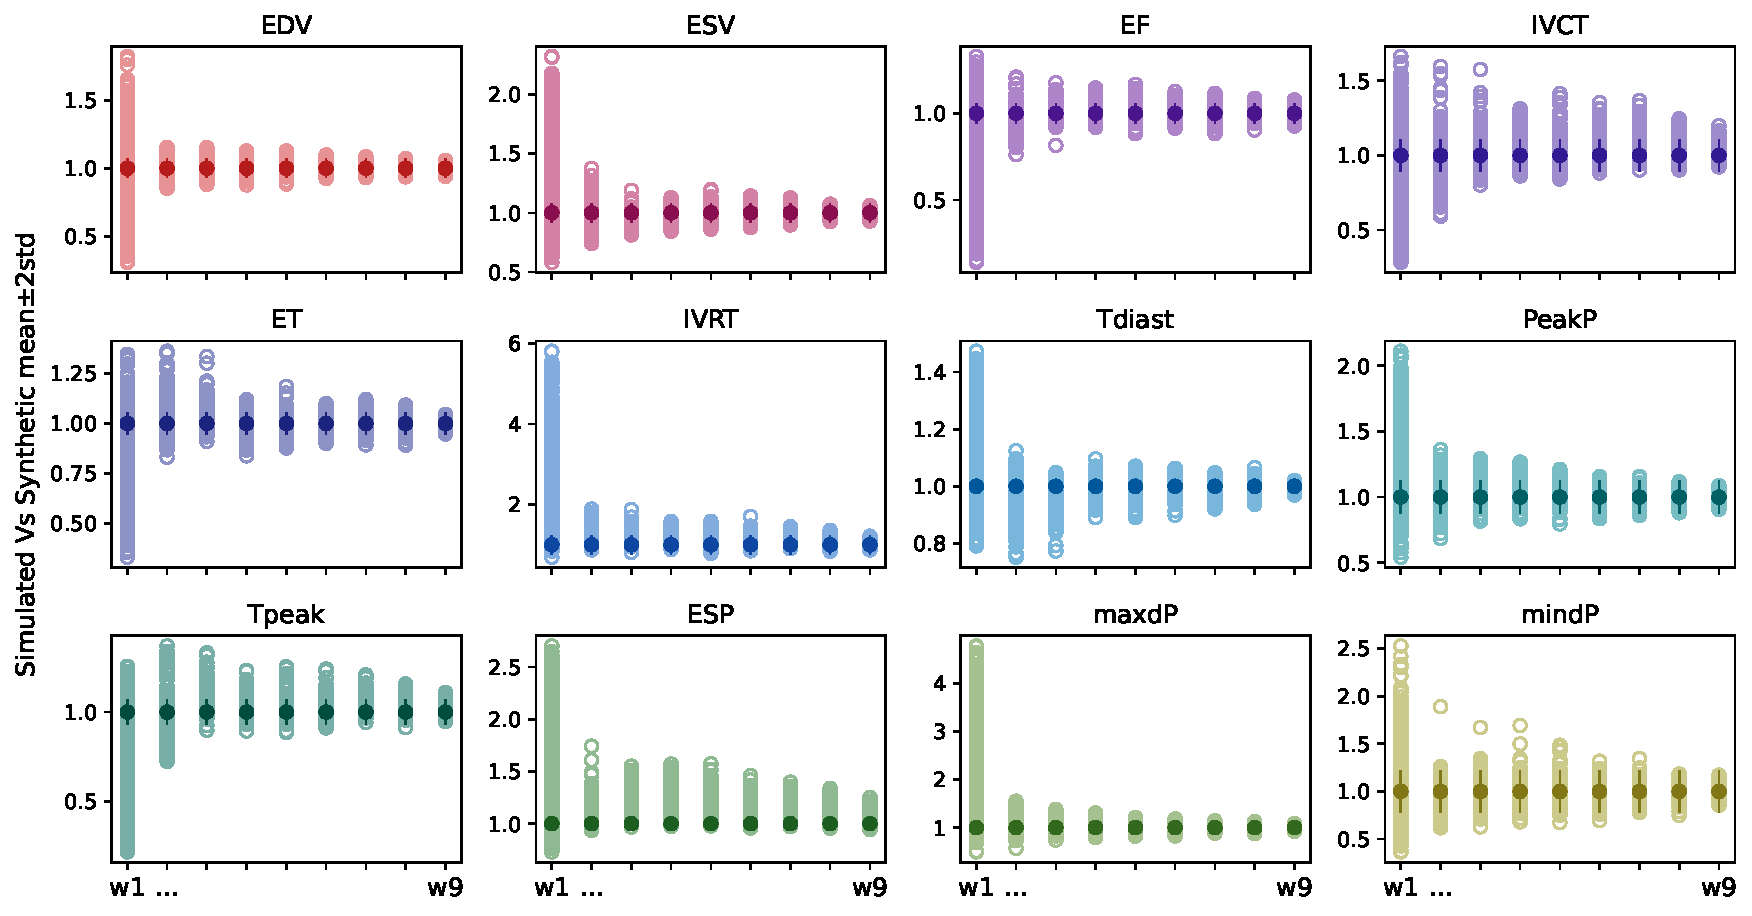
\includegraphics[width=1\textwidth]{figures/chapterA/hm_vs_synt_data_features.pdf}
    \caption{Simulated LV features’ distributions around synthetic mean values. These are obtained by evaluating the simulator at input parameter points belonging to the first (w$1$) up to the last (w$9$) waves of HM performed on synthetic data. Simulated features are shown as empty dots, while the related synthetic mean values are displayed as full dots. $2$ STD confidence intervals are also shown as vertical straight lines centred around synthetic mean values. All the displayed values (including confidence intervals) are normalised by their respective synthetic mean values.}
    \label{fig:syntfeatmatch}
\end{figure}

\vspace{0.2cm}\noindent
Moreover, we can see that the input parameters' ranges characterising the non-implausible $X_{NIMP}$ space of the last HM wave were most of the time restricted to ranges which have non-empty intersection with the ranges where the synthetic data were sampled from (Figure~\ref{fig:syntintmatch}). This shows that HM technique not only matched the target features' values but also recovered the initial sample space.

\begin{figure}[ht!]
    \myfloatalign
    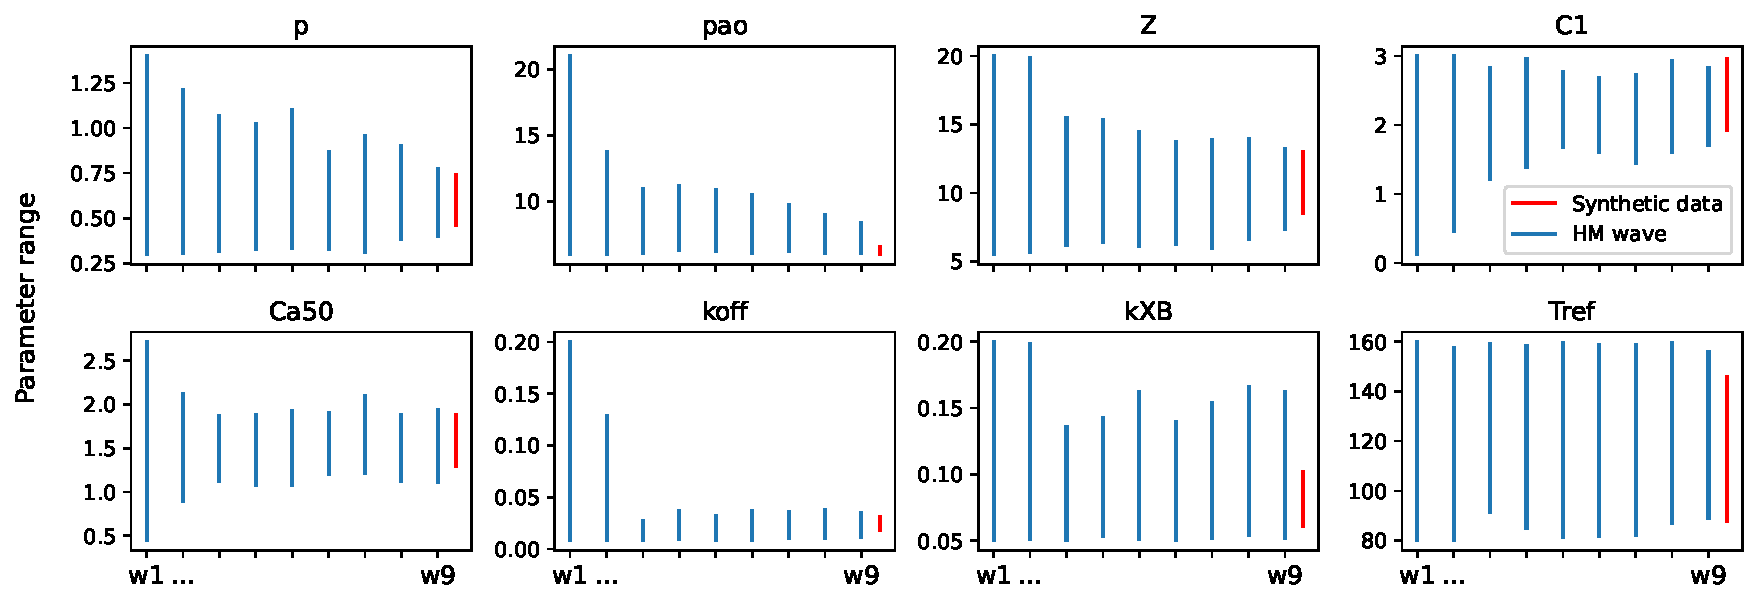
\includegraphics[width=1\textwidth]{figures/chapterA/hm_vs_synt_data_parameters.pdf}
    \caption{Input parameters' ranges at each wave during SHAM rat heart model HM on synthetic data (blue). The parameters' ranges where the synthetic data were sampled from are also shown (red).}
    \label{fig:syntintmatch}
\end{figure}

\begin{figure}[ht!]
    \myfloatalign
    \subfloat[The initial space with wave $4$ and wave $8$ $X_{NIMP}$ spaces is highlighted.]
    {\label{fig:hm1}
    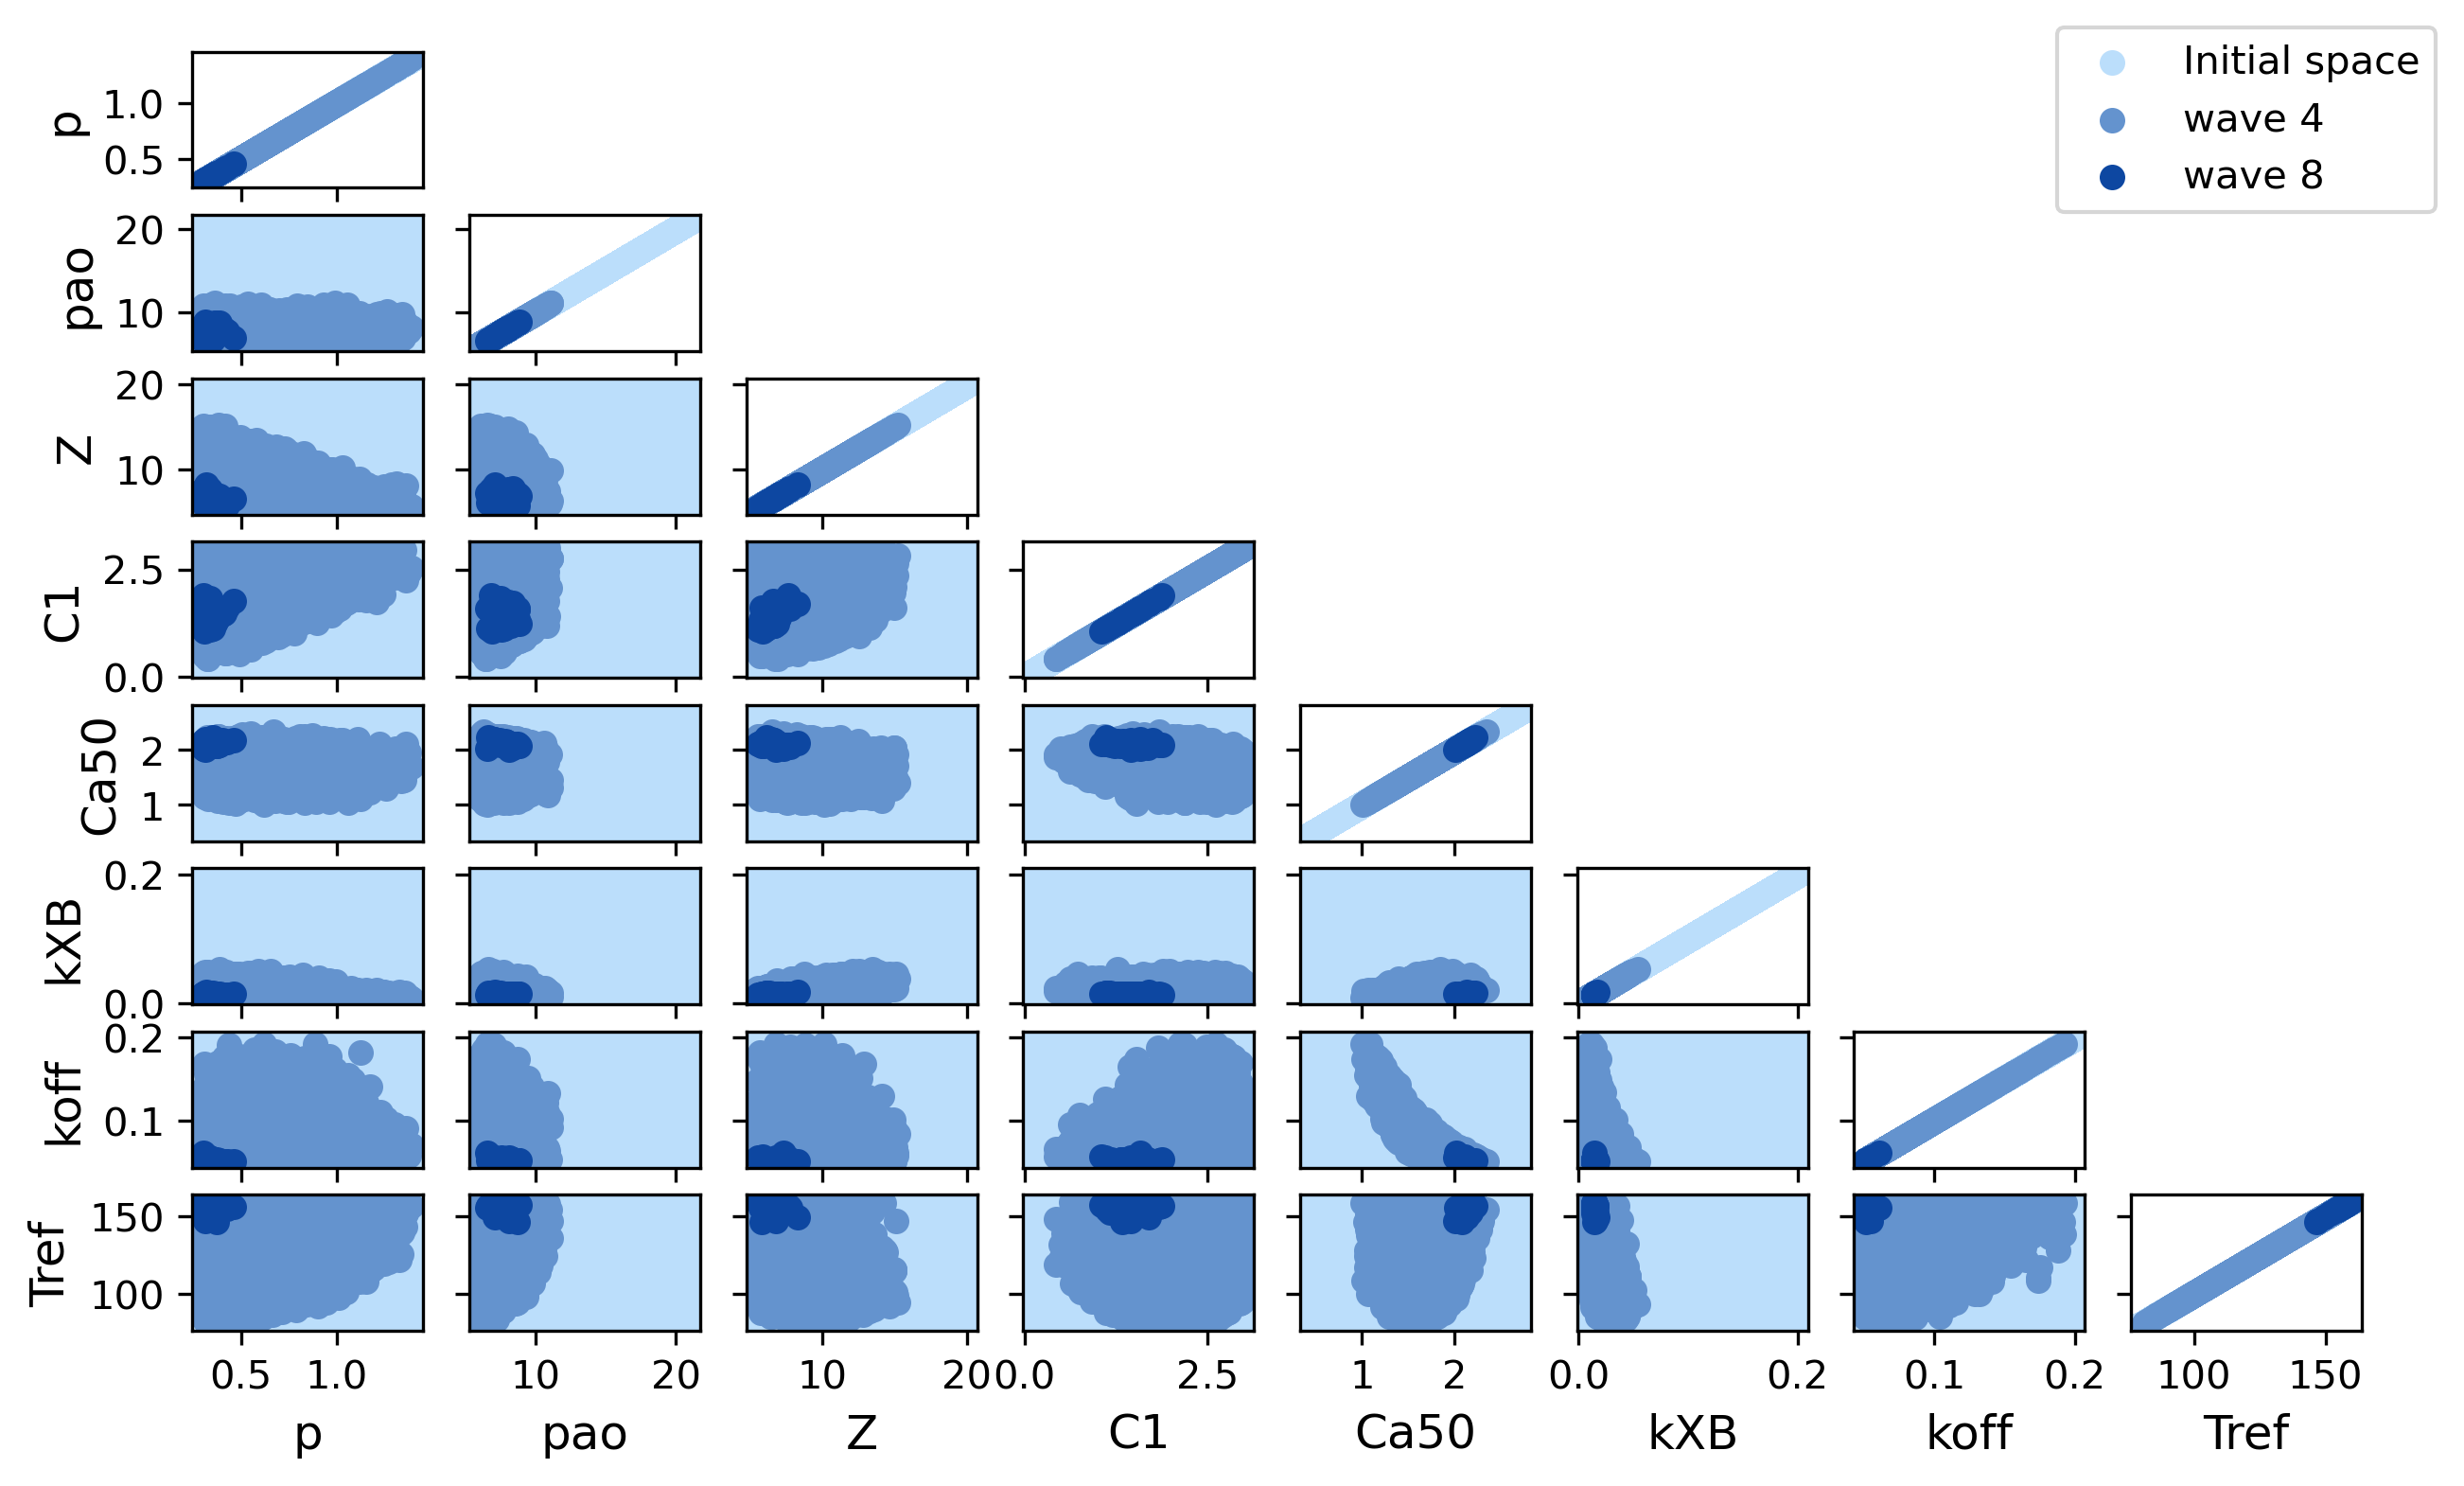
\includegraphics[width=\linewidth]{figures/chapterA/1_initial_w4_w8.png}}\quad
    \subfloat[Wave $8$ $X_{NIMP}$ space is cut out of the full space.]
    {\label{fig:hm2}
    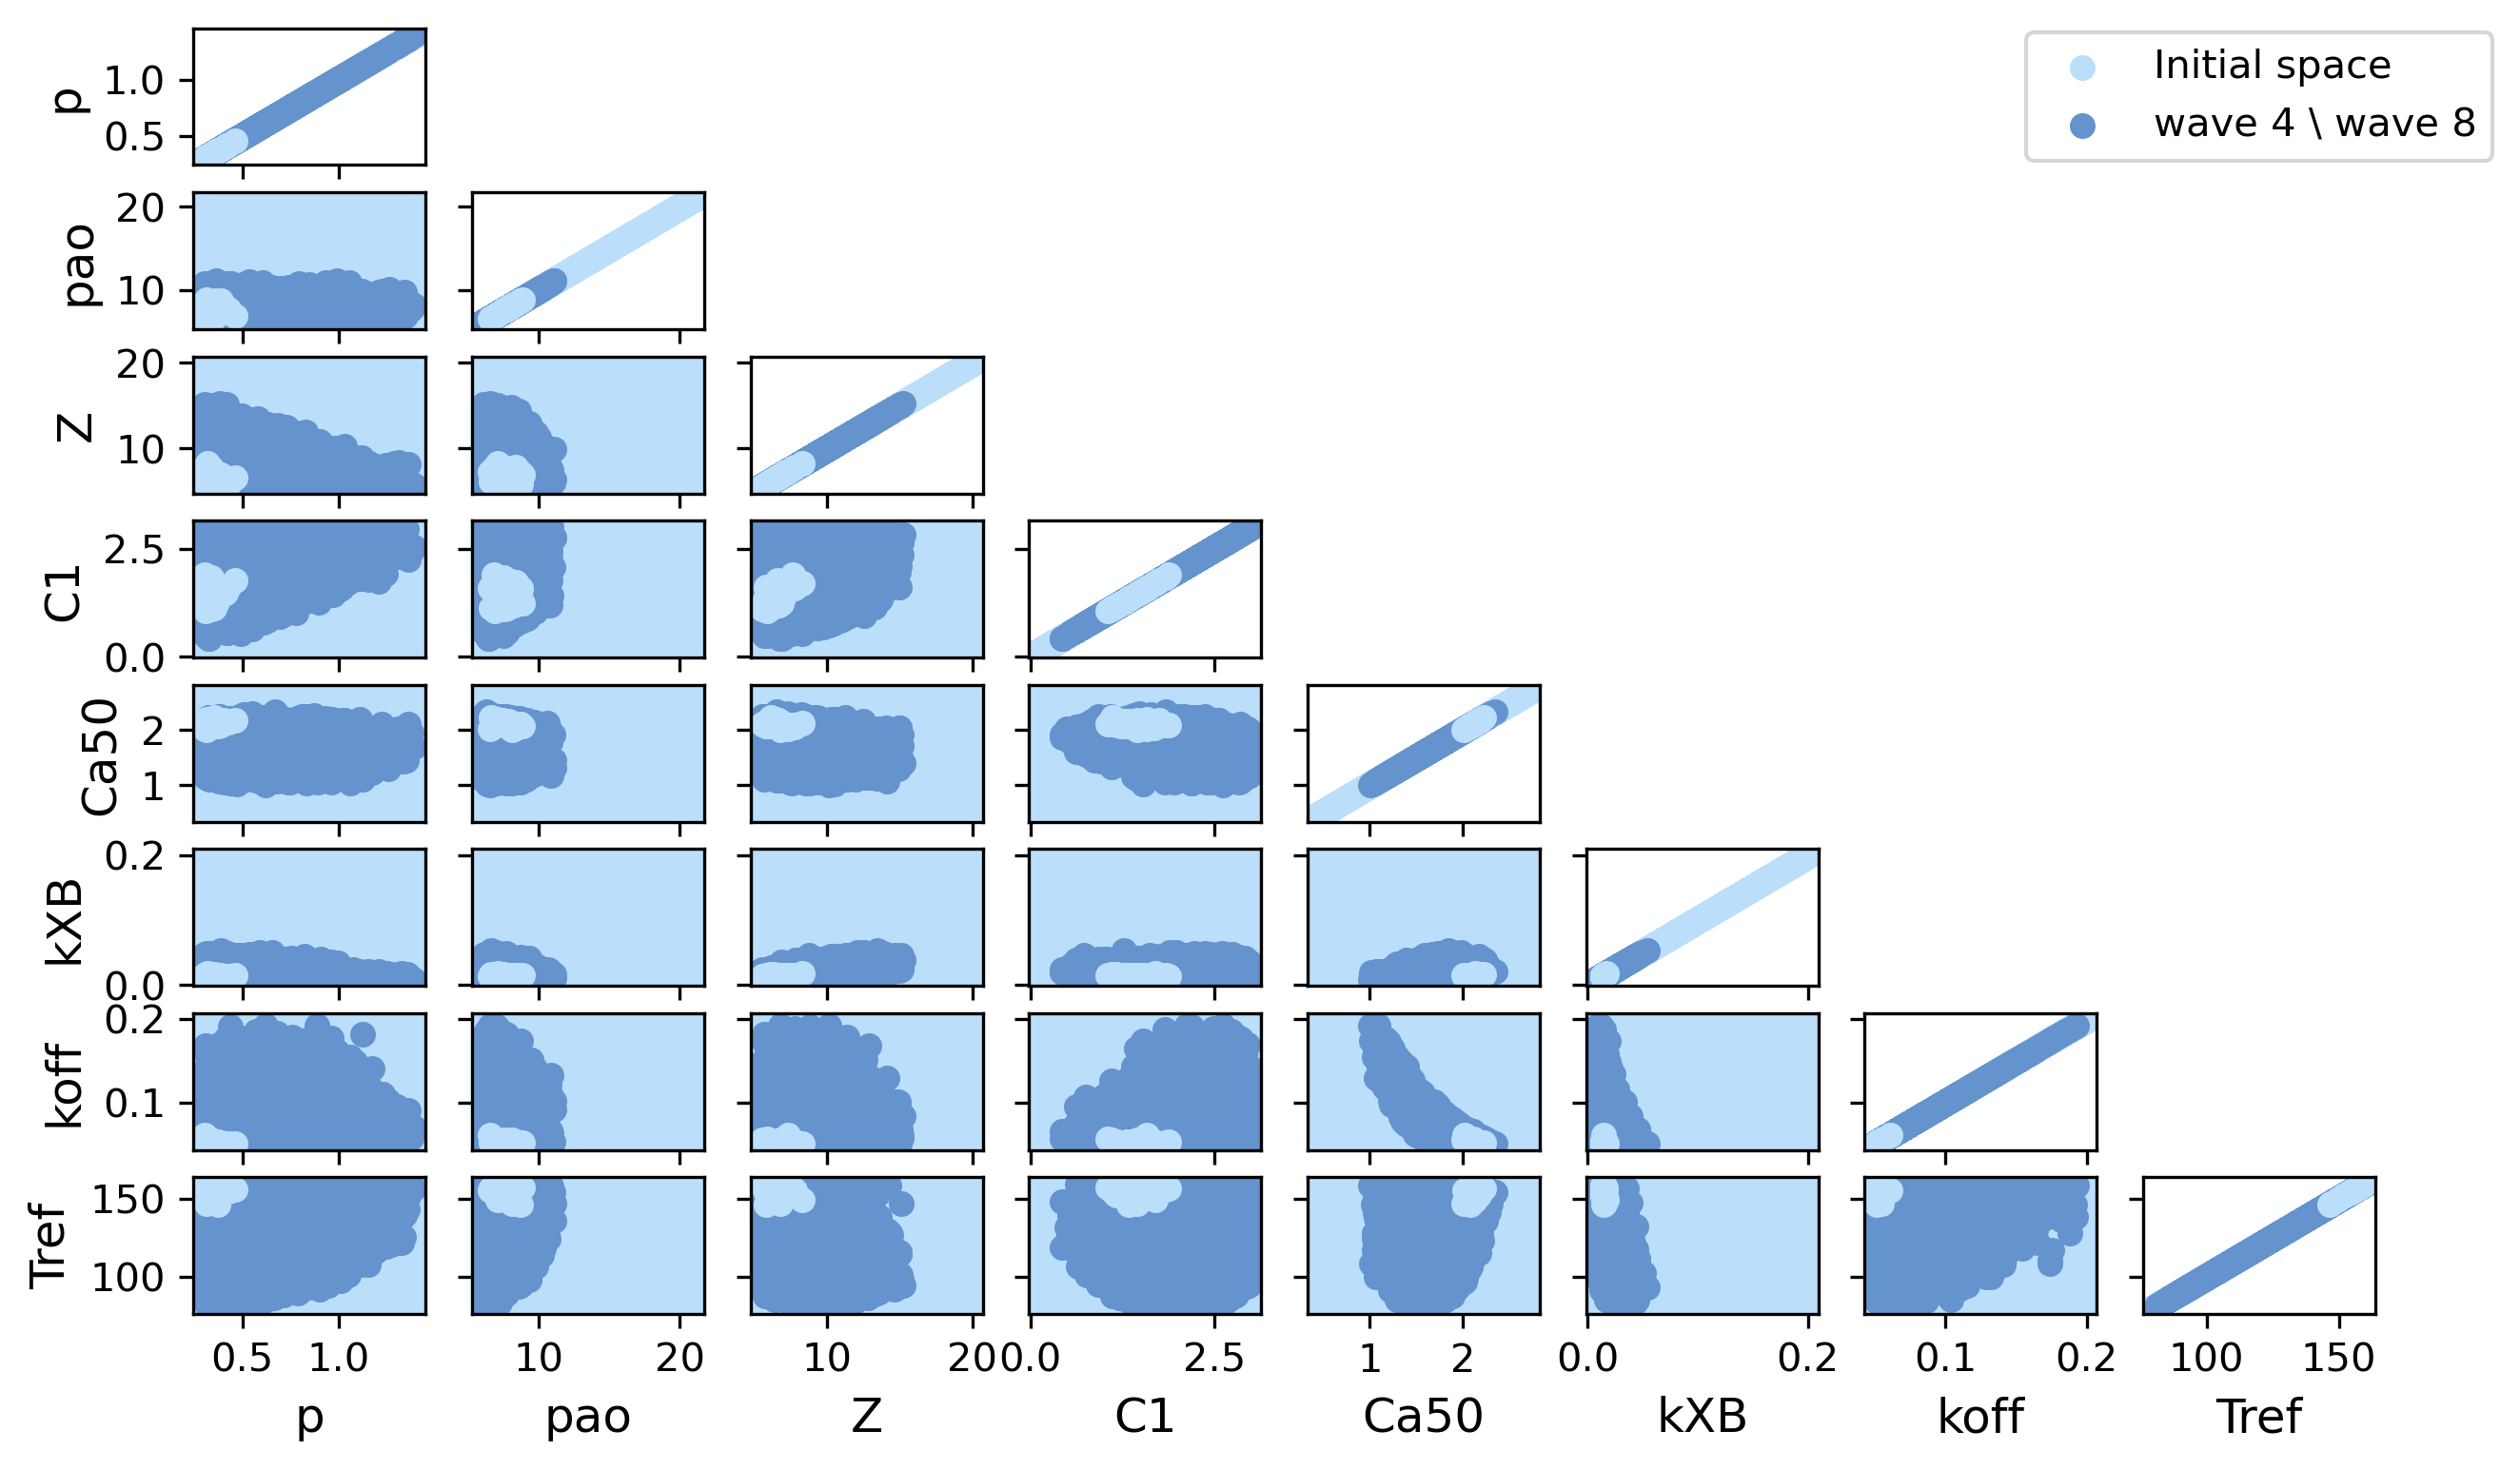
\includegraphics[width=\linewidth]{figures/chapterA/2_initial_w4minusw8.png}}\quad
    \subfloat[Points are sampled within wave $4$ $X_{NIMP}$ but not within wave $8$ $X_{NIMP}$ space.]
    {\label{fig:hm3}
    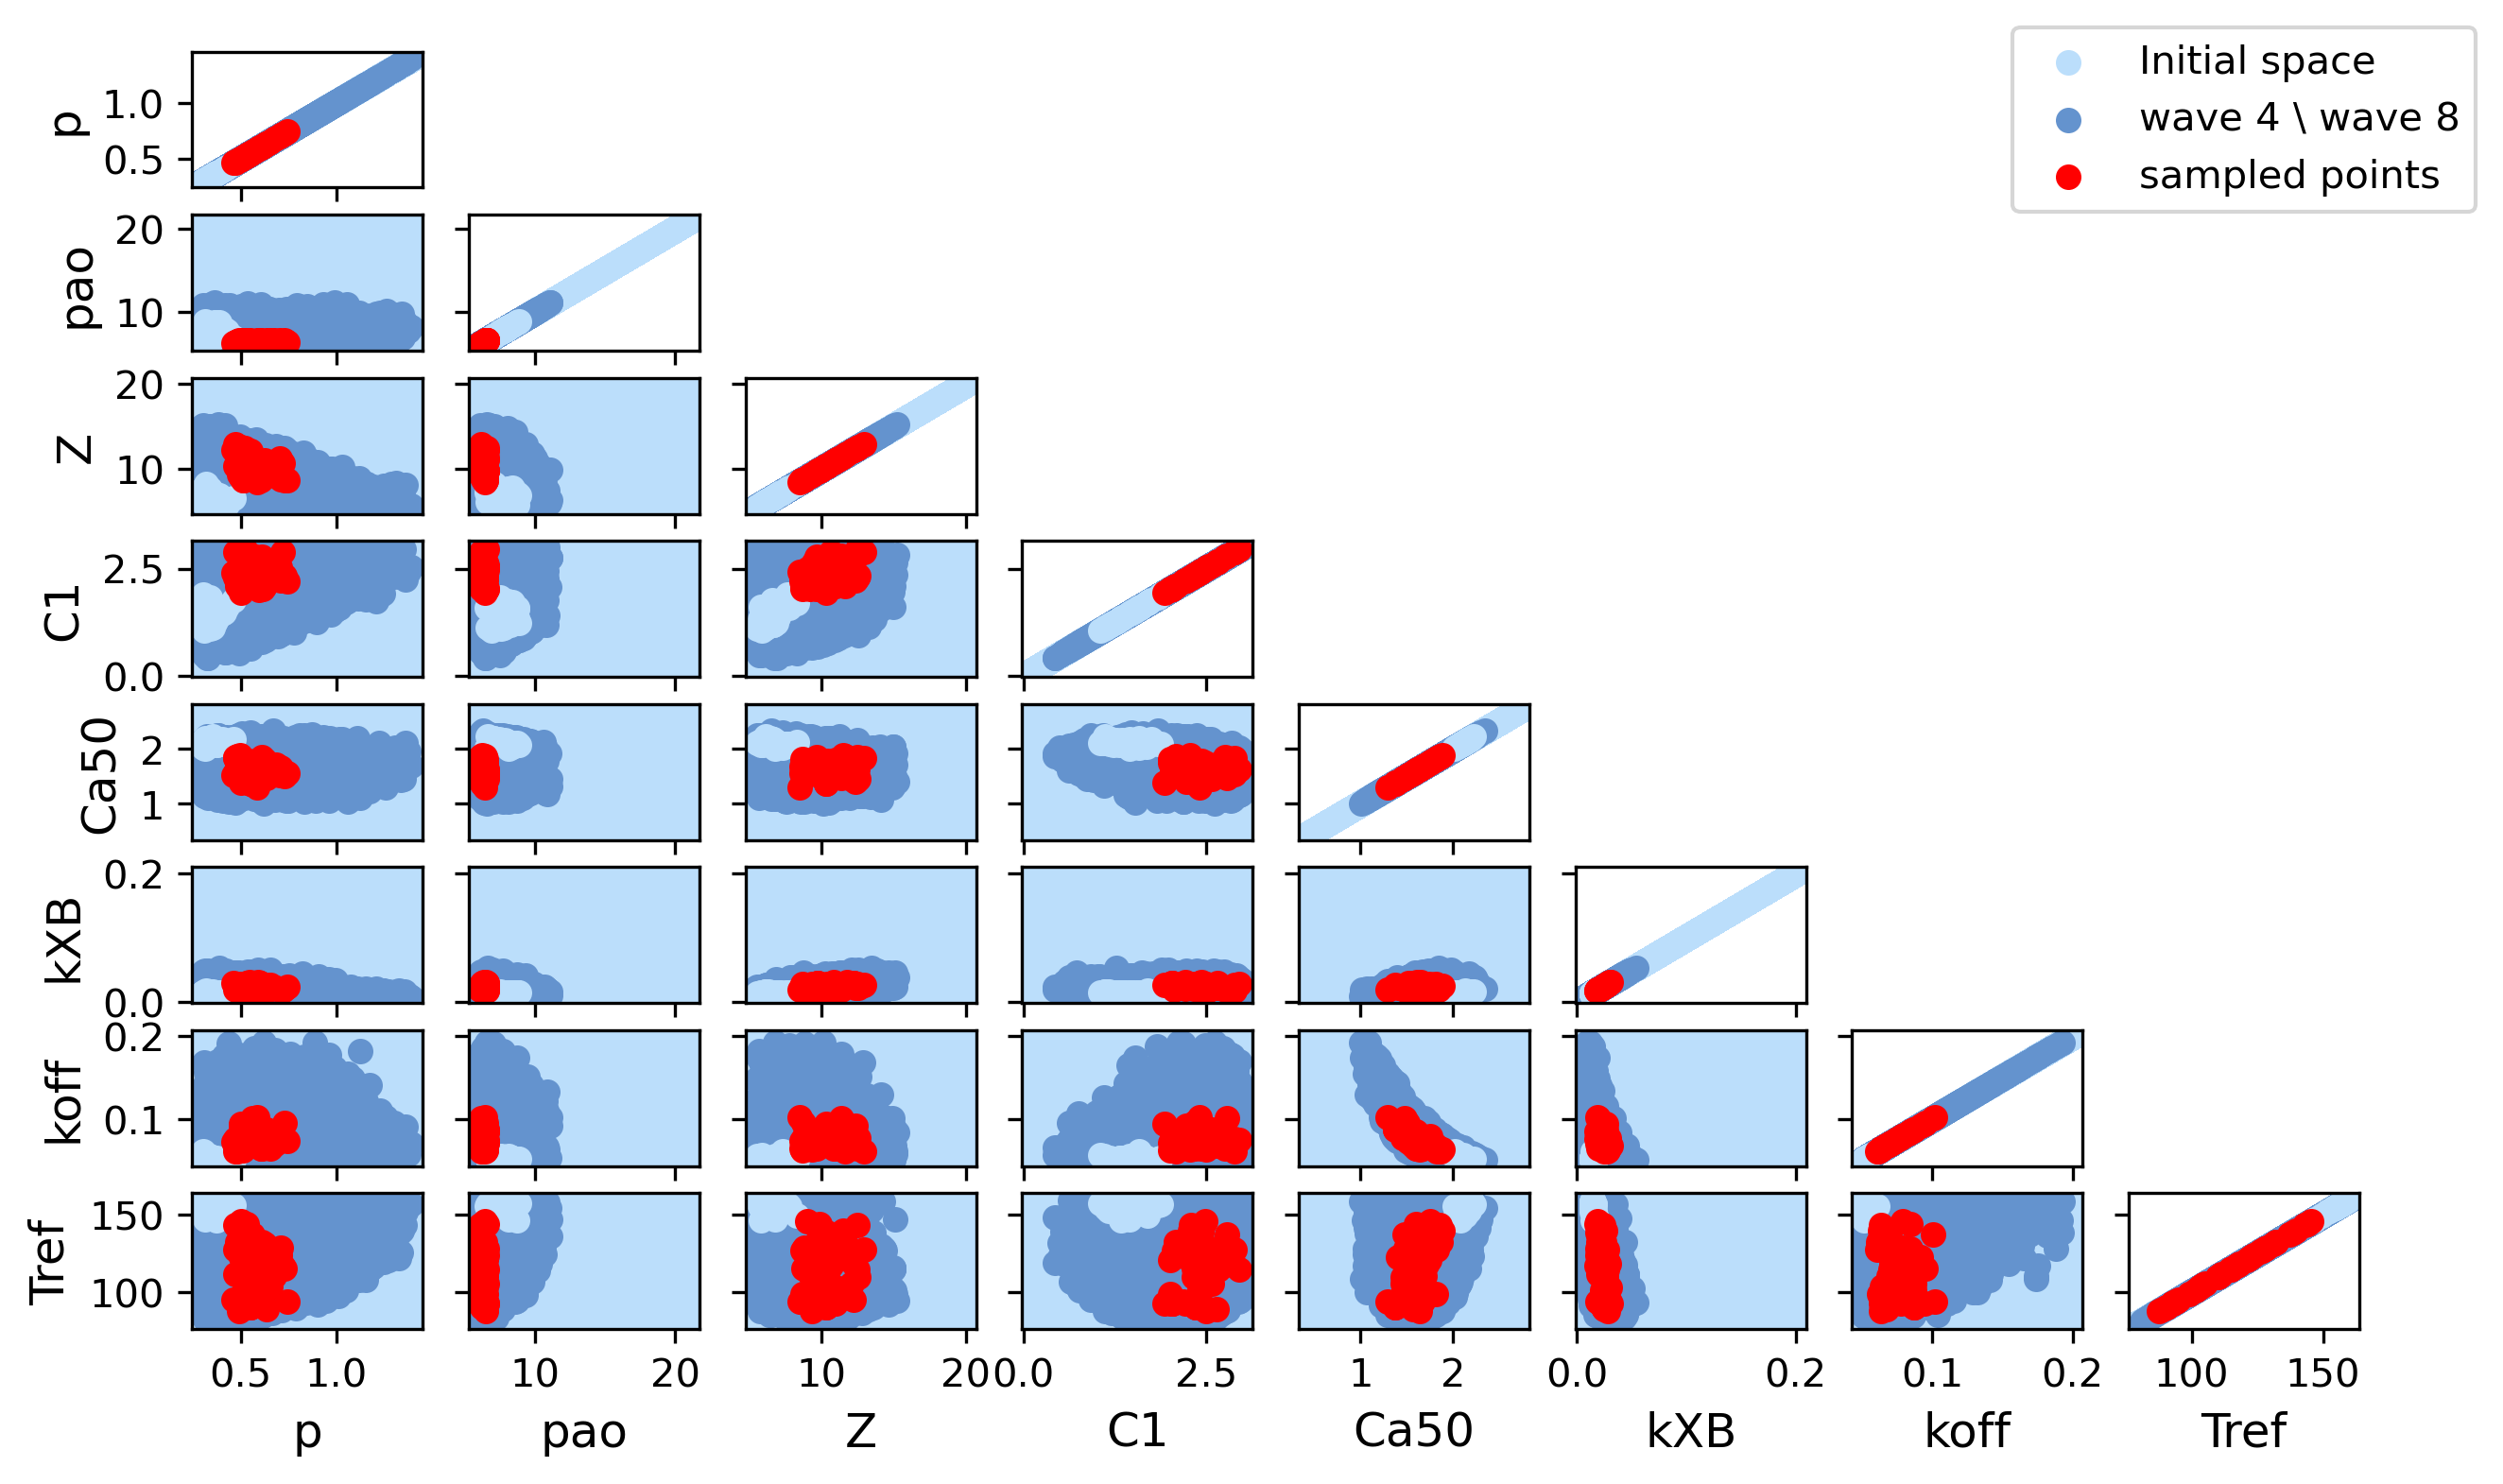
\includegraphics[width=\linewidth]{figures/chapterA/3_initial_w4minusw8_sampledpoints.png}}
    \caption{The process of points' selection for synthetic data generation to be used for HM technique validation.}\label{fig:ratrepimag}
\end{figure}